\documentclass[crop,tikz]{standalone}

\usetikzlibrary{calc}

\newcommand{\rad}{1.5}

\begin{document}
    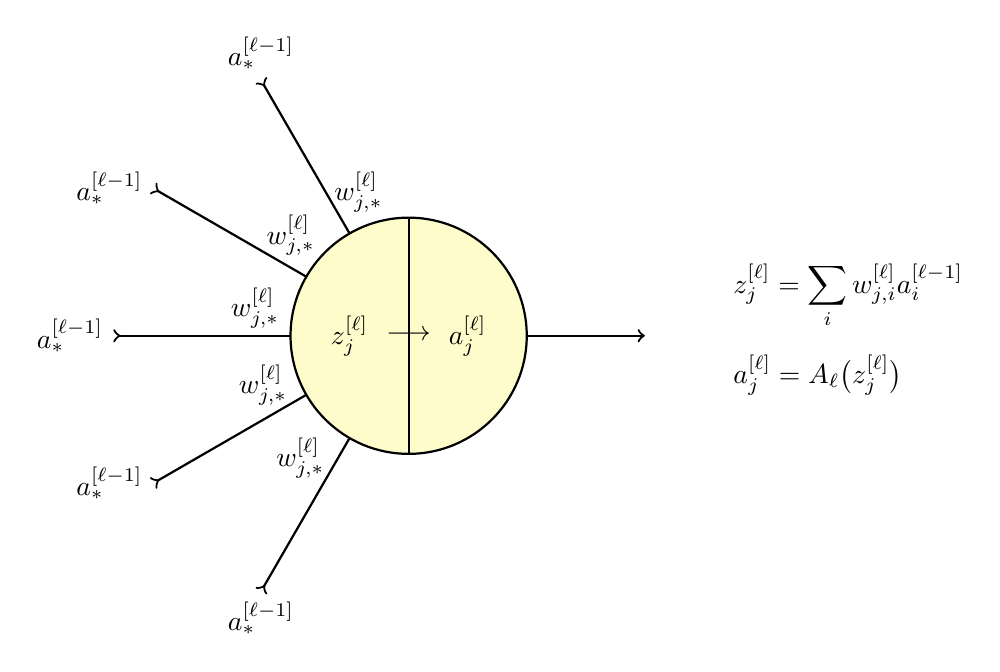
\begin{tikzpicture}
        \draw[thick, >-] ({2.5*\rad*cos(120)}, {2.5*\rad*sin(120)}) node[above] {$a^{[\ell - 1]}_*$}
        -- (0, 0);
        \draw[thick, >-] ({2.5*\rad*cos(150)}, {2.5*\rad*sin(150)}) node[left] {$a^{[\ell - 1]}_*$}
        -- (0, 0);
        \draw[thick, >-] ({2.5*\rad*cos(180)}, {2.5*\rad*sin(180)}) node[left] {$a^{[\ell - 1]}_*$}
        -- (0, 0);
        \draw[thick, >-] ({2.5*\rad*cos(210)}, {2.5*\rad*sin(210)})  node[left] {$a^{[\ell - 1]}_*$}
        -- (0, 0);
        \draw[thick, >-] ({2.5*\rad*cos(240)}, {2.5*\rad*sin(240)})  node[below] {$a^{[\ell - 1]}_*$}
        -- (0, 0);

        \draw[thick, ->] (0, 0) -- ({2*\rad}, 0);

        \node at ({1.25*\rad*cos(120) + 0.3}, {1.25*\rad*sin(120) + 0.2}) {$w^{[\ell]}_{j, *}$};
        \node at ({1.5*\rad*cos(150) + 0.45}, {1.5*\rad*sin(150) + 0.15}) {$w^{[\ell]}_{j, *}$};
        \node at ({1.3*\rad*cos(180)}, {1.1*\rad*sin(180) + 0.35}) {$w^{[\ell]}_{j, *}$};
        \node at ({1.5*\rad*cos(210) + 0.1}, {1.5*\rad*sin(210) + 0.5}) {$w^{[\ell]}_{j, *}$};
        \node at ({1.5*\rad*cos(240) - 0.25}, {1.5*\rad*sin(240) + 0.4}) {$w^{[\ell]}_{j, *}$};


        \draw[thick, fill=yellow!20] (0,0) circle (\rad);
        \draw[thick] (0, \rad) -- (0, -\rad);
        \node at (-\rad/2, 0) {$z^{[\ell]}_j$};
        \node at (0, 0) {$\longrightarrow$};
        \node at (\rad/2, 0) {$a^{[\ell]}_j$};

        \node[right] at (4, 0.5) {$\displaystyle{z_j^{[\ell]} = \sum_i w_{j, i}^{[\ell]}a_i^{[\ell - 1]}}$};
        \node[right] at (4, -0.5) {$\displaystyle{a_j^{[\ell]} = A_\ell\big(z_j^{[\ell]}\big)}$};
    \end{tikzpicture}
\end{document}